
\section{La Cybersecurity nelle Startup fintech: Sfide, Vulnerabilità e Strategie di Protezione in un Ecosistema in Rapida Evoluzione}

Il settore fintech rappresenta oggi una delle aree più dinamiche e innovative dell'ecosistema startup, con investimenti globali che hanno raggiunto i 115 miliardi di dollari, in crescita esponenziale rispetto ai 53.2 miliardi del 2018 \cite{gartnerfintech}. Questo rapido sviluppo, caratterizzato dall'implementazione di tecnologie emergenti per i servizi finanziari, porta con sé non solo opportunità senza precedenti, ma anche significative sfide in termini di sicurezza informatica. Le startup fintech, che si trovano all'intersezione tra finanza tradizionale e innovazione tecnologica, gestiscono dati estremamente sensibili, diventando bersagli privilegiati per i cybercriminali. La presente tesi esplora le vulnerabilità specifiche di queste realtà, analizza le principali minacce che esse affrontano e propone strategie di sicurezza efficaci anche in contesti di risorse limitate. Si evidenzia come un approccio proattivo alla cybersecurity non rappresenti un costo, bensì un investimento strategico fondamentale per il successo a lungo termine di una piccola-media impresa nel campo del fintech.

\subsection{Definizione di fintech}

Il termine \textit{fintech} (acronimo di ``financial technology'') identifica, nell'ecosistema economico-finanziario contemporaneo, l'intersezione tra servizi finanziari e tecnologie digitali avanzate. Esso è caratterizzato dall'implementazione di soluzioni tecnologiche innovative per la trasformazione digitale del settore bancario e finanziario \cite{tecnofinanza}. Una \textit{startup fintech} si configura come un'entità imprenditoriale emergente che opera nell'ambito della tecnologia finanziaria, sviluppando modelli di business innovativi basati su architetture tecnologiche all'avanguardia e paradigmi operativi che sfidano le metodologie consolidate delle aziende o delle organizzazioni nel settore finanziario tradizionale \cite{fintech_numeri}.

Queste organizzazioni, orientate alla tecnologia, si caratterizzano per l'adozione di approcci centrati sui dati e sul cliente (\textit{data-centric} e \textit{customer-centric}), finalizzati all'ottimizzazione dell'accessibilità, dell'efficienza operativa e della qualità dell'esperienza utente nei servizi finanziari. Esse assumono un ruolo strategico di primo piano nel processo di trasformazione digitale dell'ecosistema finanziario nazionale, contribuendo significativamente alla modernizzazione delle infrastrutture di pagamento e dei servizi bancari digitali \cite{tecnofinanza}.

Il panorama dei servizi finanziari sta subendo una profonda trasformazione, guidata dall'emergere delle startup fintech (Financial Technology) e Insurtech (Insurance Technology). Queste entità introducono modelli di business e soluzioni tecnologiche che si pongono in diretta competizione, e talvolta in collaborazione, con gli operatori tradizionali del settore. L'offerta tipica di tali startup si articola in diverse aree chiave, ciascuna caratterizzata da un elevato grado di innovazione e digitalizzazione:

\begin{figure}[htbp]
\centering
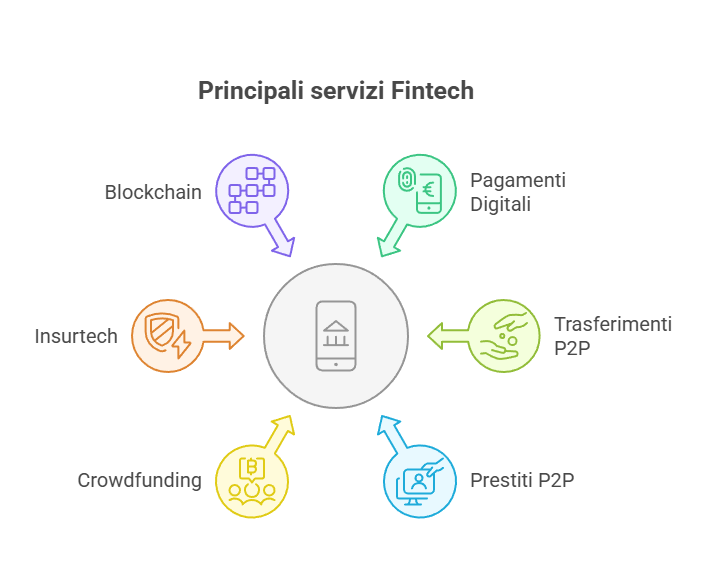
\includegraphics[width=0.9\textwidth]{fintech_services_categories}
\caption{Categorie di Servizi fintech}
\label{fig:fintech_services}
\end{figure}

\begin{itemize}
    \item \textbf{Pagamenti Digitali}: I pagamenti digitali consistono in sistemi che consentono la transazione di denaro in formato elettronico, frequentemente mediante applicazioni mobili, portafogli digitali e tecnologie contactless. Tali soluzioni mirano a migliorare l'efficienza dell'esperienza utente, ridurre i costi di transazione e velocizzare i tempi di elaborazione. Dal punto di vista della sicurezza informatica, l'infrastruttura deve prevedere meccanismi robusti di autenticazione degli utenti, crittografia end-to-end e sistemi antifrode intelligenti, per garantire la protezione dei dati e delle transazioni \cite{zhang2020digital}.
    
    \item \textbf{Trasferimenti di Denaro Peer-to-Peer (P2P)}: I sistemi \textit{Peer-to-Peer (P2P)}, che permettono il trasferimento diretto di fondi tra utenti senza l'intermediazione di istituzioni finanziarie tradizionali, consentono la riduzione dei costi e dei tempi di trasferimento. Le piattaforme devono tuttavia implementare processi rigorosi di verifica dell'identità (\textit{Know Your Customer}, KYC) e controllo antiriciclaggio (\textit{Anti-Money Laundering}, AML), oltre a misure per la protezione dei dati personali e per la prevenzione di frodi e attività illecite \cite{zhang2020digital}.
    
    \item \textbf{Prestiti Diretti tra Privati (P2P Lending)}: Questo modello di credito consente l'incontro diretto tra richiedenti e finanziatori, riducendo il ruolo delle banche. Le piattaforme si avvalgono di algoritmi di scoring basati su \textit{machine learning} e analisi dei \textit{big data} per valutare il merito creditizio. Le criticità principali riguardano la trasparenza algoritmica, la protezione dei dati finanziari sensibili e la gestione del rischio di insolvenza \cite{milne2016p2p}.
    
    \item \textbf{Finanziamento Partecipativo (Crowdfunding)}: Le piattaforme di \textit{crowdfunding} facilitano la raccolta di fondi da un'ampia base di investitori per progetti imprenditoriali, culturali o sociali. Le principali tipologie includono equity-based, lending-based, reward-based e donation-based. Le sfide di sicurezza si concentrano sulla prevenzione delle frodi, sulla protezione degli investitori e sulla trasparenza delle informazioni fornite dai promotori \cite{hornuf2018crowdfunding}.
    
    \item \textbf{Servizi Assicurativi Innovativi (Insurtech)}: L'insurtech introduce tecnologie come l'intelligenza artificiale, l'\textit{Internet of Things (IoT)} e la \textit{big data analytics} nel settore assicurativo, allo scopo di personalizzare i prodotti, migliorare la gestione dei sinistri e ottimizzare la valutazione del rischio. La protezione dei dati sensibili (ad esempio, dati sanitari o comportamentali) è una priorità, richiedendo tecniche avanzate di \textit{data governance} e sicurezza informatica \cite{eling2018insurtech}.
    
    \item \textbf{Tecnologie Blockchain e Criptovalute}: L'impiego delle \textit{Distributed Ledger Technologies (DLT)}, come la blockchain, ha rivoluzionato i servizi finanziari attraverso la decentralizzazione, la tokenizzazione di asset e la nascita della finanza decentralizzata (\textit{Decentralized Finance}, DeFi). Le sfide principali riguardano la sicurezza degli \textit{smart contract}, la custodia delle chiavi private, la prevenzione di attacchi come il 51\% attack e la conformità a regolamenti AML e di contrasto al finanziamento del terrorismo (\textit{Combating the Financing of Terrorism}, CFT) \cite{catalini2016blockchain}.
\end{itemize}

A conferma della crescente rilevanza e della dinamicità di questo settore a livello globale, anche il panorama italiano evidenzia una significativa espansione. Nel 2023, si registravano oltre 600 startup attive nei segmenti fintech e Insurtech \cite{fintech_numeri}. Questo dato sottolinea non solo la vitalità dell'ecosistema innovativo nazionale, ma anche la progressiva adozione di queste nuove soluzioni da parte del mercato. Ciò implica una crescente superficie di attacco potenziale e la necessità di strategie di cybersecurity adeguate a proteggere sia le infrastrutture di questi nuovi attori sia i dati dei loro utenti.

\subsection{Il Contesto delle Startup fintech: Un Ecosistema Dinamico e Sfidante}

Le startup fintech operano in un ambiente caratterizzato da elevata incertezza, risorse limitate e necessità di crescita rapida, fattori che influenzano profondamente le decisioni in ambito IT e sicurezza informatica \cite{fintechChallenges}. A differenza delle istituzioni finanziarie tradizionali, queste realtà innovative non dispongono generalmente di strutture gerarchiche complesse o budget consistenti dedicati alla sicurezza, dovendo invece adottare approcci agili e flessibili.

Il contesto finanziario in cui operano le startup fintech impone pressioni significative sulle decisioni di spesa. Ogni investimento, compreso quello per l'infrastruttura IT e la sicurezza, deve essere attentamente valutato in termini di ritorno immediato e benefici a lungo termine \cite{fintechChallenges}. Questa ottimizzazione dei costi rappresenta una sfida continua, poiché la sicurezza informatica richiede investimenti costanti, spesso non producendo risultati immediatamente visibili; la sua assenza, tuttavia, può comportare conseguenze catastrofiche. In questo equilibrio delicato, le startup fintech devono trovare il giusto compromesso tra la necessità di scalare rapidamente e l'implementazione di solide misure di protezione.

\subsection{Banche Tradizionali vs. Startup fintech: Divergenze Strategiche in Tecnologia, Regolamentazione e Cybersecurity}
Il panorama dei servizi finanziari è caratterizzato da una marcata eterogeneità tra gli operatori tradizionali e le nuove realtà fintech. Queste differenze si manifestano in modo sostanziale negli approcci tecnologici adottati, nei quadri normativi di riferimento e, di conseguenza, nelle strategie implementate per la cybersecurity.

Un aspetto cruciale di distinzione risiede proprio nell'approc\-cio alla cyber\-security.
Le istituzioni bancarie tradizionali operano in un contesto altamente strutturato e rigorosamente regolamentato, con precisi obblighi legali in materia di sicurezza e protezione dei dati.
Consapevoli che anche il minimo incidente può comportare la perdita di migliaia di clienti e sanzioni finanziarie significative, esse investono ingenti risorse nel testare costantemente le proprie misure di sicurezza.
Al contrario, le startup fintech hanno storicamente beneficiato di una maggiore flessibilità normativa \cite{bankingVsfintech}. Spesso nate come realtà agili e in rapida espansione, talvolta fungono da "overlay" per le banche, facilitando la fornitura di servizi finanziari innovativi pur operando, almeno inizialmente, con regolamentazioni meno stringenti. Questa disparità normativa sta tuttavia diminuendo, specialmente per quelle fintech che evolvono verso modelli bancari più completi, assoggettandosi così a un crescente scrutinio regolamentare. La sfida per queste startup consiste quindi nel bilanciare l'agilità operativa con l'adozione di standard di sicurezza elevati, anticipando l'evoluzione normativa del settore.
\newline

Queste divergenze in ambito cybersecurity sono profondamente radicate in più ampi e distinti approcci alla tecnologia e al contesto regolamentare, che riflettono modelli organizzativi e strategie di innovazione differenti.
Le banche tradizionali operano tipicamente con infrastrutture IT complesse e stratificate nel tempo, risultando spesso meno agili e più costose da aggiornare rispetto alle soluzioni moderne. La loro evoluzione tecnologica è stata prevalentemente incrementale, focalizzata sull'automazione dei processi esistenti per migliorare l'efficienza, piuttosto che su innovazioni disruptive. Storicamente, esse hanno perseguito un approccio olistico, integrando internamente un'ampia gamma di servizi, sebbene si osservi una crescente tendenza all'outsourcing e alla specializzazione. I costi IT rappresentano una quota significativa dei loro costi totali (15-20\%), a causa della complessità delle infrastrutture legacy. Sul piano regolamentare, sono soggette a un quadro normativo estremamente rigido, intensificatosi dopo la crisi finanziaria del 2008, che comporta elevati costi di compliance e ha storicamente costituito una barriera all'entrata per nuovi competitor.
Le startup fintech, d'altra parte, si contraddistinguono per l'adozione di tecnologie moderne quali big data, cloud computing e blockchain, utilizzate per creare prodotti, servizi e modelli di business innovativi, come piattaforme di crowdfunding o assicurazioni peer-to-peer. La loro innovazione non si limita a miglioramenti incrementali, ma spesso mira a ridefinire radicalmente la catena del valore esistente, come nel caso dei pagamenti peer-to-peer tramite blockchain. Molte fintech si specializzano in nicchie specifiche, bypassando attori tradizionali e promuovendo la disintermediazione; raramente offrono un ventaglio completo di servizi bancari. La tecnologia è anche un driver per modelli di business innovativi, come i robo-advisors, e per l'ingresso di nuovi player nel mercato, come le grandi aziende tecnologiche. Sul fronte regolamentare, esse possono beneficiare di iniziative volte a ridurre le barriere all'entrata, quali i cosiddetti "\textit{fintech sandbox}", che permettono di testare soluzioni in ambienti controllati. Il quadro normativo per le fintech è ancora in evoluzione, creando incertezze ma anche opportunità, con l'emergere di soluzioni "\textit{RegTech}" (Regulatory Technology) per semplificare la compliance. Questo contesto, tendenzialmente più flessibile, consente alle fintech di esercitare una significativa pressione competitiva sulle banche tradizionali \cite{puschmann_fintech_2017}.

\subsection{Analisi delle Sfide di Cybersecurity per le Startup fintech}

L'ecosistema fintech, pur essendo un catalizzatore di innovazione nel settore finanziario, presenta per le startup che ne fanno parte un panorama di sfide di cybersecurity intrinsecamente complesso. La natura agile, la focalizzazione sulla rapida immissione sul mercato (\textit{time-to-market}) e le risorse spesso limitate di queste nuove realtà imprenditoriali possono portare a una sottovalutazione della postura di sicurezza, rendendole bersagli appetibili per attori malevoli. A differenza delle istituzioni finanziarie consolidate, che dispongono di budget e team dedicati alla mitigazione dei rischi informatici, le startup fintech devono bilanciare l'innovazione con la necessità imprescindibile di proteggere dati sensibili e infrastrutture critiche.

Le principali vulnerabilità e sfide operative per le startup fintech in ambito cybersecurity possono essere così sintetizzate:

\begin{itemize}
    \item \textbf{Allocazione Iniziale delle Risorse e Priorità Strategiche}: 
    \begin{itemize}
        \item Nelle fasi embrionali, la priorità delle startup fintech è spesso concentrata sullo sviluppo del prodotto, sull'acquisizione di utenti e sulla generazione di entrate.
        \item Questa focalizzazione può marginalizzare l'integrazione di solide pratiche di cybersecurity sin dalle prime fasi di progettazione, un approccio noto come \textit{security by design}.
        \item L'assenza di figure dedicate come il \textit{Chief Information Security Officer (CISO)} e un approccio reattivo – attendere una violazione prima di intervenire – espone l'organizzazione a rischi significativi che potrebbero comprometterne la continuità operativa e la reputazione \cite{Kaur2021}.
        \item La pressione competitiva per innovare rapidamente, superando gli operatori tradizionali, può incentivare cicli di sviluppo accelerati a scapito della robustezza della sicurezza dei sistemi e delle tecnologie sottostanti \cite{teppoKauppinenRiskAndSecurityManagementInSaaSStartup_2024}.
    \end{itemize}
    
    \item \textbf{Vincoli di Budget e Competenze Specialistiche}:
    \begin{itemize}
        \item Le risorse finanziarie limitate costituiscono una barriera significativa all'adozione di soluzioni di cybersecurity avanzate.
        \item La capacità di attrarre e trattenere talenti specializzati in sicurezza informatica è limitata.
        \item Questo divario rispetto alle grandi istituzioni finanziarie, capaci di investimenti ingenti, si traduce in una potenziale disparità nella capacità di difesa contro minacce sofisticate.
    \end{itemize}
    
    \item \textbf{Gestione di Dati Finanziari Altamente Sensibili}:
    \begin{itemize}
        \item Le startup fintech trattano quotidianamente un volume considerevole di dati finanziari sensibili, inclusi dettagli di conti bancari, informazioni di identificazione personale (\textit{Personally Identifiable Information}, PII) e cronologie delle transazioni.
        \item La compromissione di tali dati non solo comporta severe sanzioni normative e perdite finanziarie dirette, ma erode irrimediabilmente la fiducia dei clienti, elemento vitale per la sostenibilità del business.
    \end{itemize}
    
    \item \textbf{Superficie di Attacco Derivante da Tecnologie Emergenti e Interconnessioni}:
    \begin{itemize}
        \item L'adozione spinta di tecnologie innovative
        (cloud computing, API aperte, intelligenza artificiale, blockchain)\allowbreak{} %
        è un tratto distintivo delle fintech.

        \item Sebbene queste tecnologie offrano vantaggi competitivi, esse introducono anche nuove superfici di attacco e vettori di minaccia \cite{fintechChallenges}.
        \item La dipendenza da servizi cloud, pur garantendo scalabilità e accessibilità, può amplificare i rischi se le configurazioni non sono gestite secondo i principi di minima esposizione e sicurezza.
        \item L'interconnessione con sistemi di terze parti (fornitori, partner) espande la superficie di attacco, rendendo cruciale una rigorosa gestione del rischio della catena di approvvigionamento (\textit{supply chain risk management}).
    \end{itemize}
    
    \item \textbf{Complessità del Panorama Normativo e degli Standard di Sicurezza}:
    \begin{itemize}
        \item Gli standard di cybersecurity esistenti sono spesso stati concepiti per istituzioni finanziarie tradizionali o contesti tecnologici più generalisti.
        \item Le specificità delle startup fintech – agilità, uso intensivo di cloud e API, modelli decentralizzati – richiedono un adattamento e un'interpretazione sartoriale di tali framework.
        \item Questo aggiunge un ulteriore livello di complessità operativa e di compliance.
    \end{itemize}
    
    \item \textbf{Minacce Interne (Insider Threats)}:
    \begin{itemize}
        \item Particolarmente nelle fasi iniziali, caratterizzate da controlli interni meno formalizzati e da una cultura organizzativa più aperta, il rischio associato a dipendenti negligenti, o in rari casi malintenzionati, non può essere trascurato.
        \item La mancanza di segregazione dei compiti (\textit{Segregation of Duties}) e di meccanismi di monitoraggio granulare degli accessi può facilitare incidenti di sicurezza originati dall'interno.
    \end{itemize}
\end{itemize}
Queste sfide strutturali e operative aumentano la vulnerabilità delle startup fintech a una varietà di attacchi informatici, rendendo essenziale l'adozione di misure di sicurezza proattive e mirate per mitigare tali rischi.

\subsection{Principali Vettori di Attacco e Minacce Informatiche nel Contesto fintech}

Il settore fintech, data la sua natura digitale e la preziosità dei dati trattati, è un obiettivo primario per una vasta gamma di cyberattacchi \cite{cyberThreatsfintech}. Tra le minacce più rilevanti per le startup fintech si annoverano:

\begin{figure}[htbp]
    \centering
    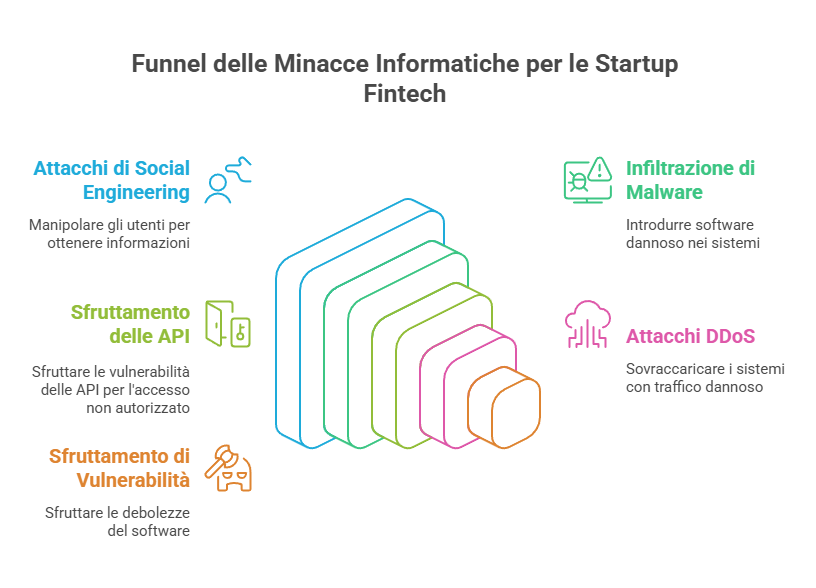
\includegraphics[width=0.9\textwidth]{cyber_threats_fintech}
    \caption{Principali vettori di attacco e minacce informatiche nel contesto fintech}
    \label{fig:cyber_threats}
\end{figure}

\begin{itemize}
    \item \textbf{Attacchi di Social Engineering e Phishing}: Tecniche come il \textit{social engineering} (ingegneria sociale) e il \textit{phishing} mirano a manipolare gli utenti o i dipendenti per indurli a rivelare credenziali di accesso, dati sensibili o a eseguire azioni malevole. E-mail, messaggi e siti web fraudolenti, che replicano comunicazioni legittime, sono strumenti comuni per compromettere la sicurezza a livello umano \cite{cyberThreatsfintech}.
    
    \item \textbf{Malware e Ransomware}: L'infiltrazione di software malevolo (\textit{malware}), inclusi i \textit{ransomware} che cifrano i dati rendendoli inaccessibili e richiedono un riscatto, rappresenta una minaccia critica. Per una startup, le cui risorse finanziarie sono limitate, l'impatto di un attacco ransomware – in termini di interruzione operativa, costi di ripristino e potenziale pagamento del riscatto – può essere particolarmente devastante \cite{cyberThreatsfintech}.
    
    \item \textbf{Vulnerabilità delle API e Configurazioni Cloud Errate}: Le \textit{Application Programming Interfaces (API)} sono fondamentali per l'ecosistema fintech, abilitando l'integrazione tra servizi diversi. Tuttavia, API insicure o mal configurate possono diventare gateway per accessi non autorizzati a dati e funzionalità critiche \cite{fintechChallenges}. Analogamente, errori nella configurazione dei servizi cloud (\textit{cloud misconfigurations}) possono esporre involontariamente dati sensibili o creare falle di sicurezza sfruttabili.
    
    \item \textbf{Attacchi Distributed Denial-of-Service (DDoS)}: Questi attacchi, noti come \textit{Distributed Denial-of-Service (DDoS)}, mirano a rendere i servizi online inaccessibili sovraccaricando l'infrastruttura target con un volume elevato di traffico malevolo. Sebbene possano apparire meno sofisticati di altri, gli attacchi DDoS possono causare significative interruzioni di servizio, danni reputazionali e perdite economiche; talvolta fungono da diversivo per mascherare intrusioni più mirate \cite{fintechChallenges}.
    
    \item \textbf{Sfruttamento di Vulnerabilità Software e Zero-Day}: Le startup, per la rapidità di sviluppo, potrebbero non avere processi di \textit{patch management} (gestione delle patch) e \textit{vulnerability assessment} (valutazione delle vulnerabilità) altrettanto maturi quanto aziende più strutturate. Questo le espone a rischi derivanti da vulnerabilità note o, nel peggiore dei casi, da quelle non ancora divulgate (definite \textit{zero-day}).
\end{itemize}

La comprensione approfondita di queste sfide e minacce è il primo passo fondamentale per le startup fintech, al fine di poter sviluppare strategie di cybersecurity proattive ed efficaci, integrando la sicurezza come componente essenziale del proprio modello di business sin dalla sua concezione. Le conseguenze di una violazione, che spaziano da perdite finanziarie dirette a danni reputazionali, impatti normativi e perdita di fiducia da parte degli stakeholder, possono compromettere la sopravvivenza stessa della startup.

\subsection{Conseguenze degli Attacchi e Impatto sulle Startup fintech}

L'impatto di un attacco informatico su una startup fintech può essere multidimensionale e, in molti casi, esistenziale. A livello finanziario, oltre ai costi diretti per il ripristino dei sistemi e la gestione dell'incidente, vanno considerati i potenziali risarcimenti a clienti danneggiati, le sanzioni normative e l'aumento dei premi assicurativi \cite{fintechChallenges}. Tuttavia, è forse l'impatto reputazionale a rappresentare la minaccia più grave: in un settore basato sulla fiducia come quello finanziario, una violazione dei dati può comprometterne irreparabilmente l'immagine, portando alla perdita di clienti attuali e potenziali.

L'interruzione operativa conseguente a un attacco può avere effetti a catena, influenzando non solo i clienti diretti ma anche partner commerciali e fornitori \cite{fintechChallenges}. In un ecosistema interconnesso come quello fintech, l'interdipendenza tra diverse piattaforme e servizi amplifica ulteriormente l'impatto di un incidente di sicurezza, con effetti che possono estendersi ben oltre il perimetro aziendale immediato.

\subsection{Importanza di un Approccio Proattivo alla Cybersecurity}

Implementare una strategia di cybersecurity solida sin dalle prime fasi di sviluppo di una startup fintech non configura un semplice onere, bensì un investimento strategico di primaria importanza \cite{fintechChallenges}. L'adozione del paradigma "security by design" permette infatti di integrare la sicurezza in maniera organica nei processi aziendali e nel ciclo di sviluppo del prodotto, contribuendo alla significativa riduzione dei costi a lungo termine e alla minimizzazione dei rischi potenziali. Al contrario, la mancata attenzione alla sicurezza nelle fasi iniziali comporta l'accumulo di un cosiddetto \textit{security debt}, ovvero un debito tecnico in ambito sicurezza che, analogamente a un mutuo con tassi elevati, diventa progressivamente più oneroso da gestire e da ripagare nel tempo. Infine, la pressione derivante dalla necessità di accelerare lo sviluppo e di raggiungere rapidamente il mercato può portare a trascurare aspetti fondamentali della sicurezza, esacerbando ulteriormente tale debito tecnico.

Un approccio preventivo alla sicurezza risulta sempre più efficace ed economico rispetto a uno reattivo \cite{fintechChallenges}. I costi per implementare misure di sicurezza di base sono generalmente inferiori rispetto a quelli necessari per rispondere a un incidente, che possono includere non solo il ripristino dei sistemi ma anche sanzioni, risarcimenti e danni reputazionali. La cybersecurity deve quindi essere considerata come parte integrante della strategia aziendale, non come un elemento accessorio o un costo da minimizzare.

Le startup fintech devono inoltre considerare che adeguati livelli di sicurezza rappresentano spesso un requisito fondamentale per attrarre investitori e partner commerciali \cite{fintechChallenges}. Durante le fasi di \textit{due diligence}, l'analisi delle misure di sicurezza implementate è diventata una componente standard, e lacune significative in questo ambito possono compromettere opportunità di finanziamento o collaborazioni strategiche.

\subsection{Approccio Metodologico}

Il presente studio si prefigge di analizzare le sfide della cybersecurity nelle startup fintech mediante un approccio metodologico che coniuga rigore strutturale e flessibilità applicativa \cite{fintechChallenges}. Nonostante la focalizzazione su un caso di studio specifico, l'intento è distillare principi e \textit{best practice} di sicurezza trasferibili al più ampio contesto delle startup fintech, a prescindere dalla piattaforma tecnologica da esse adottata. L'approccio metodologico proposto tiene conto delle intrinseche limitazioni di risorse che caratterizzano le startup, offrendo soluzioni scalabili e capaci di evolvere in parallelo alla crescita organizzativa.

La metodologia si articola su tre direttrici fondamentali: l'identificazione delle minacce peculiari al modello di business fintech, la prioritizzazione strategica degli interventi basata sulla valutazione del rapporto rischio/beneficio, e l'implementazione di controlli di sicurezza essenziali e al contempo efficaci \cite{fintechChallenges}. Tale impostazione pragmatica è volta a conseguire un livello di protezione robusto anche in contesti di risorse contenute, concentrando gli sforzi sulle aree di maggiore criticità.
